
\documentclass{article}

\usepackage{listings}
\usepackage{color}

\definecolor{dkgreen}{rgb}{0,0.6,0}
\definecolor{gray}{rgb}{0.5,0.5,0.5}
\definecolor{mauve}{rgb}{0.58,0,0.82}

\lstset{frame=tb,
  language=c++,
  aboveskip=3mm,
  belowskip=3mm,
  showstringspaces=false,
  columns=flexible,
  basicstyle={\small\ttfamily},
  numbers=none,
  numberstyle=\tiny\color{gray},
  keywordstyle=\color{blue},
  commentstyle=\color{dkgreen},
  stringstyle=\color{mauve},
  breaklines=true,
  breakatwhitespace=true,
  tabsize=3
}

\usepackage{tikz}
\usepackage{amsthm}
\usepackage{amsfonts}
\usepackage{amsmath}
\usepackage{amssymb}
\usepackage{fullpage}
\usepackage{graphicx}
\usepackage[usenames]{color}
\usepackage{hyperref}

  \hypersetup{
    colorlinks = true,
    urlcolor = blue,       % color of external links using \href
    linkcolor= blue,       % color of internal links 
    citecolor= blue,       % color of links to bibliography
    filecolor= blue,        % color of file links
    }
    
\usepackage{listings}

\definecolor{dkgreen}{rgb}{0,0.6,0}
\definecolor{gray}{rgb}{0.5,0.5,0.5}
\definecolor{mauve}{rgb}{0.58,0,0.82}

\lstset{frame=tb,
  language=haskell,
  aboveskip=3mm,
  belowskip=3mm,
  showstringspaces=false,
  columns=flexible,
  basicstyle={\small\ttfamily},
  numbers=none,
  numberstyle=\tiny\color{gray},
  keywordstyle=\color{blue},
  commentstyle=\color{dkgreen},
  stringstyle=\color{mauve},
  breaklines=true,
  breakatwhitespace=true,
  tabsize=3
}

\theoremstyle{theorem} 
   \newtheorem{theorem}{Theorem}[section]
   \newtheorem{corollary}[theorem]{Corollary}
   \newtheorem{lemma}[theorem]{Lemma}
   \newtheorem{proposition}[theorem]{Proposition}
\theoremstyle{definition}
   \newtheorem{definition}[theorem]{Definition}
   \newtheorem{example}[theorem]{Example}
\theoremstyle{remark}    
  \newtheorem{remark}[theorem]{Remark}


\title{CPSC-402 Report\\Compiler Construction}
\author{Samuel Ellenhorn  \\ Chapman University}

\date{\today}

\begin{document}

\maketitle

\begin{abstract}
The purpose of this paper is to demonstrate my knowledge the compiler which sits behind high level code. Proper knowledge of assembly code can, in many cases lead to extreme improvements in efficiency. It is also possible that some tasks can only be completed when implemented in assembly code. 
\end{abstract}

\tableofcontents

\section{Introduction}\label{intro}



\subsection{General Remarks}
Compiler construction is an interesting course which I have enjoyed. I have found some of the assignments to be very difficult, however, after completion I have gained insight into creating more efficient code. The following report contains examples of my work throughout the year.

 

\medskip\noindent



\section{Homework}\label{homework}



\subsection{Homework 1}

\textbf{Exercise 2.2.4} Give DFA's accepting the following languages over the alpahbet {0, 1}:\\
 a) The set of all strings ending in 000\\
 
  \begin{center}
     Answer:
 \end{center}
 
 \begin{center}
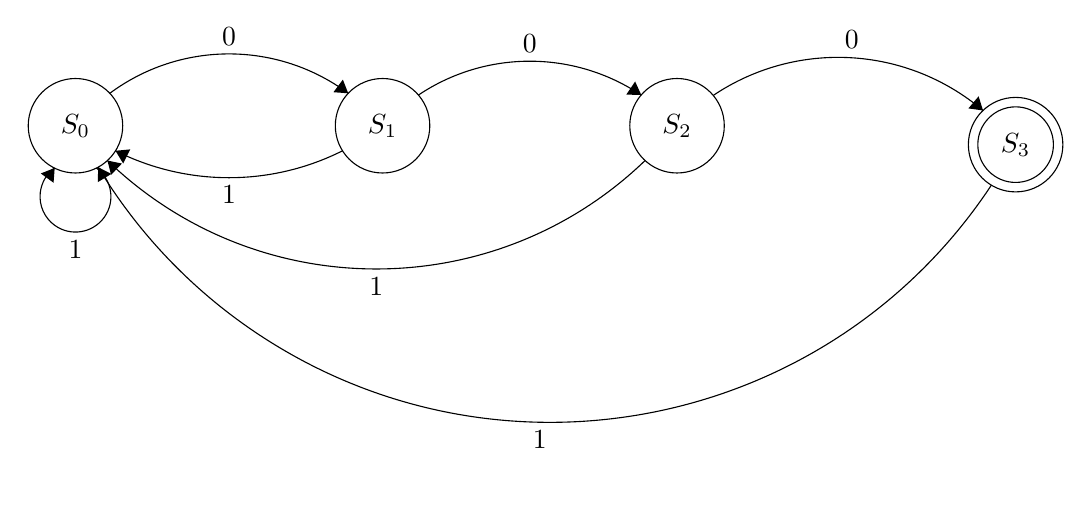
\begin{tikzpicture}[scale=0.2]
\tikzstyle{every node}+=[inner sep=0pt]
\draw [black] (22.7,-6.9) circle (3);
\draw (22.7,-6.9) node {$S_1$};
\draw [black] (41.4,-6.9) circle (3);
\draw (41.4,-6.9) node {$S_2$};
\draw [black] (62.9,-8.1) circle (3);
\draw (62.9,-8.1) node {$S_3$};
\draw [black] (62.9,-8.1) circle (2.4);
\draw [black] (3.2,-6.9) circle (3);
\draw (3.2,-6.9) node {$S_0$};
\draw [black] (24.973,-4.953) arc (123.83061:56.16939:12.712);
\fill [black] (39.13,-4.95) -- (38.74,-4.09) -- (38.18,-4.92);
\draw (32.05,-2.3) node [above] {$0$};
\draw [black] (43.695,-4.977) arc (123.92066:49.69016:14.223);
\fill [black] (60.83,-5.93) -- (60.55,-5.03) -- (59.9,-5.8);
\draw (52.49,-2.03) node [above] {$0$};
\draw [black] (4.523,-9.58) arc (54:-234:2.25);
\draw (3.2,-14.15) node [below] {$1$};
\fill [black] (1.88,-9.58) -- (1,-9.93) -- (1.81,-10.52);
\draw [black] (5.375,-4.844) arc (126.61245:53.38755:12.701);
\fill [black] (20.52,-4.84) -- (20.18,-3.97) -- (19.58,-4.77);
\draw (12.95,-1.84) node [above] {$0$};
\draw [black] (39.372,-9.108) arc (-46.05987:-133.94013:24.603);
\fill [black] (5.23,-9.11) -- (5.46,-10.02) -- (6.15,-9.3);
\draw (22.3,-16.5) node [below] {$1$};
\draw [black] (20.161,-8.489) arc (-63.30863:-116.69137:16.053);
\fill [black] (5.74,-8.49) -- (6.23,-9.3) -- (6.68,-8.4);
\draw (12.95,-10.7) node [below] {$1$};
\draw [black] (61.36,-10.673) arc (-33.46035:-148.84269:33.564);
\fill [black] (4.64,-9.53) -- (4.62,-10.48) -- (5.48,-9.96);
\draw (32.68,-26.24) node [below] {$1$};
\end{tikzpicture}
\end{center}
\\
 b)The set of all strings with three consecutive 0's(not necessarily at the end):\\
 
 \begin{center}
     Answer:
 \end{center}
 This language is described as follows:\\
 \[L = \{ w \epsilon \{0,1\}^* | w = x000y, x,y \epsilon \{0,1\}^*\}\]\\
 A DFA for this language can be seen here:\\\\
 
\begin{center}
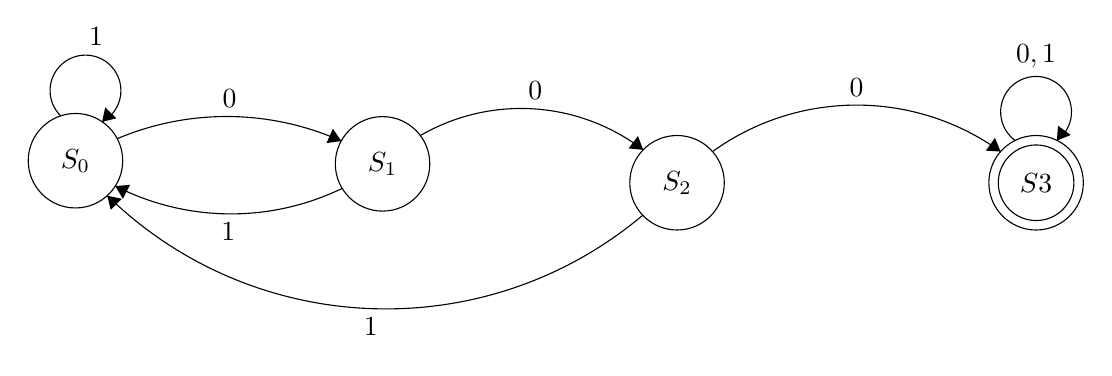
\begin{tikzpicture}[scale=0.2]
\tikzstyle{every node}+=[inner sep=0pt]
\draw [black] (22.8,-9.3) circle (3);
\draw (22.8,-9.3) node {$S_1$};
\draw [black] (41.5,-10.5) circle (3);
\draw (41.5,-10.5) node {$S_2$};
\draw [black] (3.3,-9.1) circle (3);
\draw (3.3,-9.1) node {$S_0$};
\draw [black] (64.3,-10.5) circle (3);
\draw (64.3,-10.5) node {$S3$};
\draw [black] (64.3,-10.5) circle (2.4);
\draw [black] (25.195,-7.505) arc (120.11892:52.53768:12.756);
\fill [black] (39.35,-8.41) -- (39.02,-7.53) -- (38.42,-8.32);
\draw (32.5,-5.25) node [above] {$0$};
\draw [black] (5.951,-7.703) arc (112.95612:65.86862:17.809);
\fill [black] (20.18,-7.85) -- (19.65,-7.07) -- (19.24,-7.98);
\draw (13.08,-5.78) node [above] {$0$};
\draw [black] (20.239,-10.854) arc (-64.08084:-117.09442:16.144);
\fill [black] (5.83,-10.71) -- (6.31,-11.52) -- (6.77,-10.63);
\draw (13.01,-12.99) node [below] {$1$};
\draw [black] (2.37,-6.26) arc (225.8699:-62.1301:2.25);
\draw (4.6,-1.82) node [above] {$1$};
\fill [black] (4.99,-6.63) -- (5.9,-6.41) -- (5.19,-5.71);
\draw [black] (62.977,-7.82) arc (234:-54:2.25);
\draw (64.3,-3.25) node [above] {$0,1$};
\fill [black] (65.62,-7.82) -- (66.5,-7.47) -- (65.69,-6.88);
\draw [black] (39.324,-12.562) arc (-49.92801:-134.2698:25.343);
\fill [black] (5.32,-11.32) -- (5.54,-12.23) -- (6.24,-11.52);
\draw (22.05,-19.03) node [below] {$1$};
\draw [black] (43.75,-8.523) arc (125.80308:54.19692:15.64);
\fill [black] (62.05,-8.52) -- (61.69,-7.65) -- (61.11,-8.46);
\draw (52.9,-5.07) node [above] {$0$};
\end{tikzpicture}
\end{center}




 c)The set of strings with 011 as a substring.
 
  \begin{center}
     Answer:
 \end{center}
This language is described as follows:\\
 \[L = \{ w \epsilon \{0,1\}^* | w = x0y1z1u, x,yz,u \epsilon \{0,1\}^*\}\]\\
 A DFA for this language can be seen here:\\\\


\begin{center}
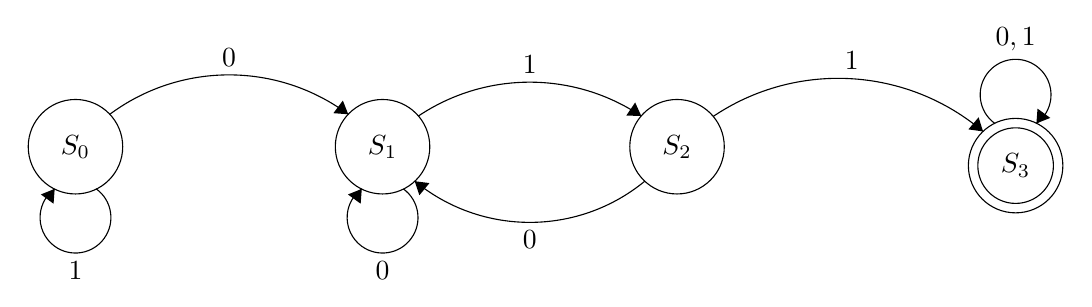
\begin{tikzpicture}[scale=0.2]
\tikzstyle{every node}+=[inner sep=0pt]
\draw [black] (22.7,-7.8) circle (3);
\draw (22.7,-7.8) node {$S_1$};
\draw [black] (41.4,-7.8) circle (3);
\draw (41.4,-7.8) node {$S_2$};
\draw [black] (62.9,-9) circle (3);
\draw (62.9,-9) node {$S_3$};
\draw [black] (62.9,-9) circle (2.4);
\draw [black] (3.2,-7.8) circle (3);
\draw (3.2,-7.8) node {$S_0$};
\draw [black] (24.973,-5.853) arc (123.83061:56.16939:12.712);
\fill [black] (39.13,-5.85) -- (38.74,-4.99) -- (38.18,-5.82);
\draw (32.05,-3.2) node [above] {$1$};
\draw [black] (61.577,-6.32) arc (234:-54:2.25);
\draw (62.9,-1.75) node [above] {$0,1$};
\fill [black] (64.22,-6.32) -- (65.1,-5.97) -- (64.29,-5.38);
\draw [black] (43.695,-5.877) arc (123.92066:49.69016:14.223);
\fill [black] (60.83,-6.83) -- (60.55,-5.93) -- (59.9,-6.7);
\draw (52.49,-2.93) node [above] {$1$};
\draw [black] (24.023,-10.48) arc (54:-234:2.25);
\draw (22.7,-15.05) node [below] {$0$};
\fill [black] (21.38,-10.48) -- (20.5,-10.83) -- (21.31,-11.42);
\draw [black] (4.523,-10.48) arc (54:-234:2.25);
\draw (3.2,-15.05) node [below] {$1$};
\fill [black] (1.88,-10.48) -- (1,-10.83) -- (1.81,-11.42);
\draw [black] (39.357,-9.985) arc (-50.54714:-129.45286:11.499);
\fill [black] (24.74,-9.99) -- (25.04,-10.88) -- (25.68,-10.11);
\draw (32.05,-13.11) node [below] {$0$};
\draw [black] (5.375,-5.744) arc (126.61245:53.38755:12.701);
\fill [black] (20.52,-5.74) -- (20.18,-4.87) -- (19.58,-5.67);
\draw (12.95,-2.74) node [above] {$0$};
\end{tikzpicture}
\end{center}




\subsection{Homework 2 with Regular Expressions}

\textbf{Exercise 2.3.4}
\\
a) The set of strings over alphabet {0,1...9} such that the final digit has appeared before.
  \begin{center}
     Answer:
 \end{center}
 
 \begin{center}
\begin{tikzpicture}[scale=0.2]
\tikzstyle{every node}+=[inner sep=0pt]
\draw [black] (3.3,-30.3) circle (3);
\draw (3.3,-30.3) node {$S_1$};
\draw [black] (32.7,-9.1) circle (3);
\draw (32.7,-9.1) node {$S_2$};
\draw [black] (32.7,-21.3) circle (3);
\draw (32.7,-21.3) node {$S_3$};
\draw [black] (31.9,-49.3) circle (3);
\draw (31.9,-49.3) node {$S_4$};
\draw [black] (59.1,-30.3) circle (3);
\draw (59.1,-30.3) node {$S_5$};
\draw [black] (59.1,-30.3) circle (2.4);
\draw [black] (31.9,-34.7) circle (3);
\draw (31.9,-34.7) node {$S_3_8$};
\draw [black] (35.04,-10.98) -- (56.76,-28.42);
\fill [black] (56.76,-28.42) -- (56.45,-27.53) -- (55.82,-28.31);
\draw (44.89,-20.19) node [below] {$0$};
\draw [black] (6.17,-29.42) -- (29.83,-22.18);
\fill [black] (29.83,-22.18) -- (28.92,-21.93) -- (29.21,-22.89);
\draw (18.85,-26.35) node [below] {$1$};
\draw [black] (5.8,-31.96) -- (29.4,-47.64);
\fill [black] (29.4,-47.64) -- (29.01,-46.78) -- (28.46,-47.61);
\draw (16.6,-40.3) node [below] {$9$};
\draw [black] (34.36,-47.58) -- (56.64,-32.02);
\fill [black] (56.64,-32.02) -- (55.7,-32.07) -- (56.27,-32.89);
\draw (46.5,-40.3) node [below] {$9$};
\draw [black] (5.73,-28.55) -- (30.27,-10.85);
\fill [black] (30.27,-10.85) -- (29.33,-10.92) -- (29.91,-11.73);
\draw (19,-20.2) node [below] {$0$};
\draw [black] (35.54,-22.27) -- (56.26,-29.33);
\fill [black] (56.26,-29.33) -- (55.66,-28.6) -- (55.34,-29.55);
\draw (45,-26.33) node [below] {$1$};
\draw [black] (31.377,-6.42) arc (234:-54:2.25);
\draw (32.7,-1.85) node [above] {$0,1...9$};
\fill [black] (34.02,-6.42) -- (34.9,-6.07) -- (34.09,-5.48);
\draw [black] (31.377,-18.62) arc (234:-54:2.25);
\draw (32.7,-14.05) node [above] {$0,1...9$};
\fill [black] (34.02,-18.62) -- (34.9,-18.27) -- (34.09,-17.68);
\draw [black] (30.5,-46.2) -- (30.67,-46.57);
\fill [black] (30.67,-46.57) -- (30.79,-45.63) -- (29.88,-46.04);
\draw [black] (30.577,-46.62) arc (234:-54:2.25);
\draw (31.9,-42.05) node [above] {$0,1...9$};
\fill [black] (33.22,-46.62) -- (34.1,-46.27) -- (33.29,-45.68);
\draw [black] (1.977,-27.62) arc (234:-54:2.25);
\draw (3.3,-23.05) node [above] {$0,1...9$};
\fill [black] (4.62,-27.62) -- (5.5,-27.27) -- (4.69,-26.68);
\draw [black] (6.27,-30.76) -- (28.93,-34.24);
\fill [black] (28.93,-34.24) -- (28.22,-33.63) -- (28.07,-34.62);
\draw (16.89,-33.17) node [below] {$2-8$};
\draw [black] (34.86,-34.22) -- (56.14,-30.78);
\fill [black] (56.14,-30.78) -- (55.27,-30.41) -- (55.43,-31.4);
\draw (46.27,-33.17) node [below] {$2-8$};
\draw [black] (30.577,-32.02) arc (234:-54:2.25);
\draw (31.9,-27.45) node [above] {$0,1...9$};
\fill [black] (33.22,-32.02) -- (34.1,-31.67) -- (33.29,-31.08);
\end{tikzpicture}
\end{center}

Regular Expressions: \\\(\{0+...9\}^*(0\{0+...9\}^*0+...9)\)



b) The set of strings over alphabet {0,1...9} the final digit has not appeared before.
  \begin{center}
     Answer:
 \end{center}
 


\begin{center}
\begin{tikzpicture}[scale=0.2]
\tikzstyle{every node}+=[inner sep=0pt]
\draw [black] (3.2,-30.3) circle (3);
\draw (3.2,-30.3) node {$S_1$};
\draw [black] (32.6,-9.1) circle (3);
\draw (32.6,-9.1) node {$S_2$};
\draw [black] (32.6,-21.7) circle (3);
\draw (32.6,-21.7) node {$S_3$};
\draw [black] (32.6,-54.8) circle (3);
\draw (32.6,-54.8) node {$S_4$};
\draw [black] (59,-30.3) circle (3);
\draw (59,-30.3) node {$S_5$};
\draw [black] (59,-30.3) circle (2.4);
\draw [black] (32.6,-42.1) circle (3);
\draw (32.6,-42.1) node {$S_3_8$};
\draw [black] (35.447,-10.045) arc (69.71122:32.75774:44.548);
\fill [black] (57.46,-27.72) -- (57.45,-26.78) -- (56.61,-27.32);
\draw (48.9,-16.6) node [above] {$0$};
\draw [black] (6.08,-29.46) -- (29.72,-22.54);
\fill [black] (29.72,-22.54) -- (28.81,-22.29) -- (29.09,-23.25);
\draw (20.37,-26.66) node [below] {$0,1...9$};
\draw [black] (5.5,-32.22) -- (30.3,-52.88);
\fill [black] (30.3,-52.88) -- (30,-51.98) -- (29.36,-52.75);
\draw (14.89,-43.04) node [below] {$0,1...9$};
\draw [black] (34.8,-52.76) -- (56.8,-32.34);
\fill [black] (56.8,-32.34) -- (55.87,-32.52) -- (56.55,-33.25);
\draw (46.82,-43.04) node [below] {$9$};
\draw [black] (5.217,-28.08) arc (136.67997:114.90991:80.431);
\fill [black] (29.86,-10.31) -- (28.92,-10.2) -- (29.34,-11.1);
\draw (13.69,-17.52) node [above] {$0,1...9$};
\draw [black] (35.45,-22.63) -- (56.15,-29.37);
\fill [black] (56.15,-29.37) -- (55.54,-28.65) -- (55.23,-29.6);
\draw (44.92,-26.54) node [below] {$1$};
\draw [black] (31.277,-6.42) arc (234:-54:2.25);
\draw (32.6,-1.85) node [above] {$0,1...9$};
\fill [black] (33.92,-6.42) -- (34.8,-6.07) -- (33.99,-5.48);
\draw [black] (31.277,-19.02) arc (234:-54:2.25);
\draw (32.6,-14.45) node [above] {$0,1...9$};
\fill [black] (33.92,-19.02) -- (34.8,-18.67) -- (33.99,-18.08);
\draw [black] (31.2,-51.7) -- (31.37,-52.07);
\fill [black] (31.37,-52.07) -- (31.49,-51.13) -- (30.58,-51.54);
\draw [black] (31.277,-52.12) arc (234:-54:2.25);
\draw (32.6,-47.55) node [above] {$0,1...9$};
\fill [black] (33.92,-52.12) -- (34.8,-51.77) -- (33.99,-51.18);
\draw [black] (5.98,-31.42) -- (29.82,-40.98);
\fill [black] (29.82,-40.98) -- (29.26,-40.22) -- (28.89,-41.15);
\draw (16.15,-36.73) node [below] {$3-8$};
\draw [black] (35.34,-40.88) -- (56.26,-31.52);
\fill [black] (56.26,-31.52) -- (55.33,-31.39) -- (55.73,-32.31);
\draw (47.59,-36.72) node [below] {$3-8$};
\draw [black] (31.277,-39.42) arc (234:-54:2.25);
\draw (32.6,-34.85) node [above] {$0,1...9$};
\fill [black] (33.92,-39.42) -- (34.8,-39.07) -- (33.99,-38.48);
\draw [black] (6.2,-30.3) -- (56,-30.3);
\fill [black] (56,-30.3) -- (55.2,-29.8) -- (55.2,-30.8);
\draw (31.1,-30.8) node [below] {$0,1...9$};
\end{tikzpicture}
\end{center}


Definitions:\\
\(\sigma_0=1+2+3+4+5+6+7+8+9\)\\
\(\sigma_1=0+2+3+4+5+6+7+8+9\)\\\\
First answer:\(\{0+...9\}^*(0\{0+...9\}0+...)\)\\
Final Answer:  \(\sigma^*0+\sigma^*1+\sigma^*2+\sigma^*3...\sigma^*9\)\\\\


c) The set of strings of 0 and 1's such that there are two 0s separated by
a number of positions that is a multiple of 4 Note that 0 is an allowable multiple of 4.
  \begin{center}
     Answer:
 \end{center}
 
\begin{center}
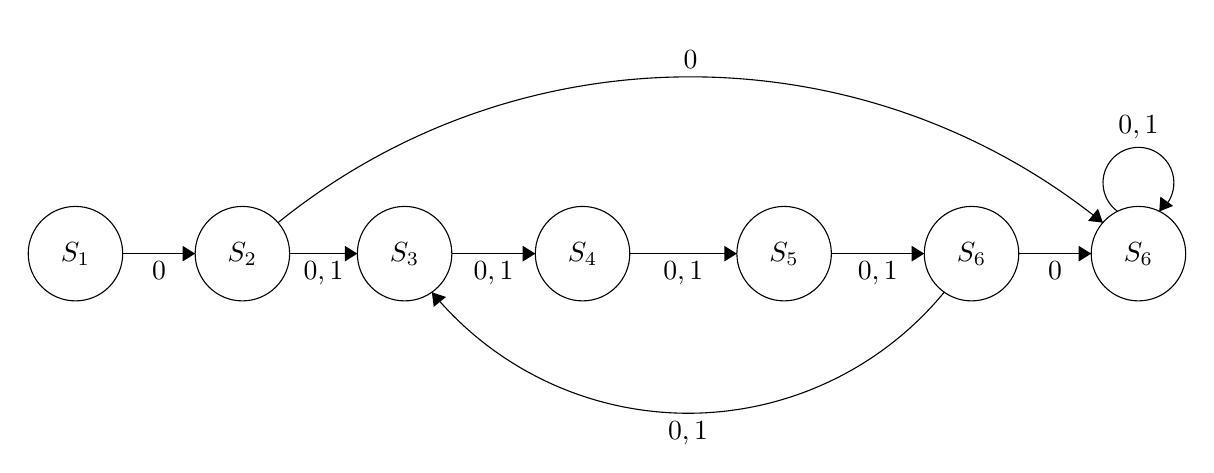
\begin{tikzpicture}[scale=0.2]
\tikzstyle{every node}+=[inner sep=0pt]
\draw [black] (3.3,-13.5) circle (3);
\draw (3.3,-13.5) node {$S_1$};
\draw [black] (13.9,-13.5) circle (3);
\draw (13.9,-13.5) node {$S_2$};
\draw [black] (24.2,-13.5) circle (3);
\draw (24.2,-13.5) node {$S_3$};
\draw [black] (35.5,-13.5) circle (3);
\draw (35.5,-13.5) node {$S_4$};
\draw [black] (48.3,-13.5) circle (3);
\draw (48.3,-13.5) node {$S_5$};
\draw [black] (60.2,-13.5) circle (3);
\draw (60.2,-13.5) node {$S_6$};
\draw [black] (70.8,-13.5) circle (3);
\draw (70.8,-13.5) node {$S_6$};
\draw [black] (6.3,-13.5) -- (10.9,-13.5);
\fill [black] (10.9,-13.5) -- (10.1,-13) -- (10.1,-14);
\draw (8.6,-14) node [below] {$0$};
\draw [black] (16.9,-13.5) -- (21.2,-13.5);
\fill [black] (21.2,-13.5) -- (20.4,-13) -- (20.4,-14);
\draw (19.05,-14) node [below] {$0,1$};
\draw [black] (51.3,-13.5) -- (57.2,-13.5);
\fill [black] (57.2,-13.5) -- (56.4,-13) -- (56.4,-14);
\draw (54.25,-14) node [below] {$0,1$};
\draw [black] (27.2,-13.5) -- (32.5,-13.5);
\fill [black] (32.5,-13.5) -- (31.7,-13) -- (31.7,-14);
\draw (29.85,-14) node [below] {$0,1$};
\draw [black] (38.5,-13.5) -- (45.3,-13.5);
\fill [black] (45.3,-13.5) -- (44.5,-13) -- (44.5,-14);
\draw (41.9,-14) node [below] {$0,1$};
\draw [black] (63.2,-13.5) -- (67.8,-13.5);
\fill [black] (67.8,-13.5) -- (67,-13) -- (67,-14);
\draw (65.5,-14) node [below] {$0$};
\draw [black] (16.163,-11.532) arc (128.95063:51.04937:41.656);
\fill [black] (68.54,-11.53) -- (68.23,-10.64) -- (67.6,-11.42);
\draw (42.35,-1.77) node [above] {$0$};
\draw [black] (69.477,-10.82) arc (234:-54:2.25);
\draw (70.8,-6.25) node [above] {$0,1$};
\fill [black] (72.12,-10.82) -- (73,-10.47) -- (72.19,-9.88);
\draw [black] (58.467,-15.946) arc (-39.40456:-140.59544:21.053);
\fill [black] (25.93,-15.95) -- (26.05,-16.88) -- (26.83,-16.25);
\draw (42.2,-24.13) node [below] {$0,1$};
\end{tikzpicture}
\end{center}

Regular Expressions: \((0+1)^* 0((0+1)(0+1)(0+1)(0+1))^*(0+1)^*\)


\textbf{Exercise 2.5.3}
\\
a) The set of strings consisting of zero or more a's followed by zero or more
b's followed by 0 or more c's
  \begin{center}
     Answer:
 \end{center}

\begin{center}
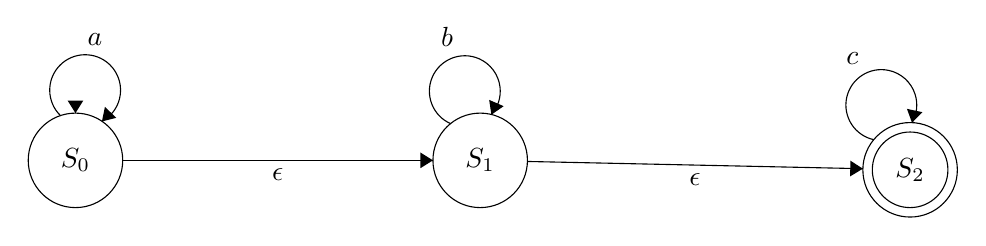
\begin{tikzpicture}[scale=0.2]
\tikzstyle{every node}+=[inner sep=0pt]
\draw [black] (3.3,-9.1) circle (3);
\draw (3.3,-9.1) node {$S_0$};
\draw [black] (29,-9.1) circle (3);
\draw (29,-9.1) node {$S_1$};
\draw [black] (56.3,-9.7) circle (3);
\draw (56.3,-9.7) node {$S_2$};
\draw [black] (56.3,-9.7) circle (2.4);
\draw [black] (3.3,-5.9) -- (3.3,-6.1);
\fill [black] (3.3,-6.1) -- (3.8,-5.3) -- (2.8,-5.3);
\draw [black] (2.356,-6.265) arc (226.14669:-61.85331:2.25);
\draw (4.53,-1.83) node [above] {$a$};
\fill [black] (4.98,-6.63) -- (5.89,-6.4) -- (5.17,-5.7);
\draw [black] (27.128,-6.771) arc (246.52881:-41.47119:2.25);
\draw (26.9,-1.93) node [above] {$b$};
\fill [black] (29.71,-6.2) -- (30.49,-5.66) -- (29.57,-5.26);
\draw [black] (54.003,-7.788) arc (257.96249:-30.03751:2.25);
\draw (52.64,-3.02) node [above] {$c$};
\fill [black] (56.42,-6.71) -- (57.08,-6.04) -- (56.1,-5.83);
\draw [black] (32,-9.17) -- (53.3,-9.63);
\fill [black] (53.3,-9.63) -- (52.51,-9.12) -- (52.49,-10.12);
\draw (42.64,-9.92) node [below] {$\epsilon$};
\draw [black] (6.3,-9.1) -- (26,-9.1);
\fill [black] (26,-9.1) -- (25.2,-8.6) -- (25.2,-9.6);
\draw (16.15,-9.6) node [below] {$\epsilon$};
\end{tikzpicture}
\end{center}



Regular Expressions: a* b* c*
\\
b) The set of strings that consist of either 01 repeated one or 010 repeated more times or repeated one or more times


\begin{center}
\begin{tikzpicture}[scale=0.2]
\tikzstyle{every node}+=[inner sep=0pt]
\draw [black] (3.3,-20.7) circle (3);
\draw (3.3,-20.7) node {$S_0$};
\draw [black] (19.1,-9.5) circle (3);
\draw (19.1,-9.5) node {$S_1$};
\draw [black] (17.7,-26) circle (3);
\draw (17.7,-26) node {$S_4$};
\draw [black] (36.9,-26) circle (3);
\draw (36.9,-26) node {$S_5$};
\draw [black] (55.4,-26) circle (3);
\draw (55.4,-26) node {$S_6$};
\draw [black] (69,-26) circle (3);
\draw (69,-26) node {$S_7$};
\draw [black] (69,-26) circle (2.4);
\draw [black] (55.4,-9.5) circle (3);
\draw (55.4,-9.5) node {$S_3$};
\draw [black] (55.4,-9.5) circle (2.4);
\draw [black] (36.9,-9.5) circle (3);
\draw (36.9,-9.5) node {$S_2$};
\draw [black] (39.9,-26) -- (52.4,-26);
\fill [black] (52.4,-26) -- (51.6,-25.5) -- (51.6,-26.5);
\draw (46.15,-26.5) node [below] {$1$};
\draw [black] (5.75,-18.97) -- (16.65,-11.23);
\fill [black] (16.65,-11.23) -- (15.71,-11.29) -- (16.29,-12.11);
\draw (12.12,-15.6) node [below] {$\epsilon$};
\draw [black] (20.7,-26) -- (33.9,-26);
\fill [black] (33.9,-26) -- (33.1,-25.5) -- (33.1,-26.5);
\draw (27.3,-26.5) node [below] {$0$};
\draw [black] (6.12,-21.74) -- (14.88,-24.96);
\fill [black] (14.88,-24.96) -- (14.31,-24.22) -- (13.96,-25.16);
\draw (9.64,-23.87) node [below] {$\epsilon$};
\draw [black] (58.4,-26) -- (66,-26);
\fill [black] (66,-26) -- (65.2,-25.5) -- (65.2,-26.5);
\draw (62.2,-26.5) node [below] {$0$};
\draw [black] (67.777,-28.738) arc (-27.20766:-152.79234:27.466);
\fill [black] (18.92,-28.74) -- (18.84,-29.68) -- (19.73,-29.22);
\draw (43.35,-44.15) node [below] {$\epsilon$};
\draw [black] (21.333,-7.499) arc (128.49231:51.50769:25.573);
\fill [black] (21.33,-7.5) -- (22.27,-7.39) -- (21.65,-6.61);
\draw (37.25,-1.44) node [above] {$\epsilon$};
\draw [black] (39.9,-9.5) -- (52.4,-9.5);
\fill [black] (52.4,-9.5) -- (51.6,-9) -- (51.6,-10);
\draw (46.15,-10) node [below] {$1$};
\draw [black] (22.1,-9.5) -- (33.9,-9.5);
\fill [black] (33.9,-9.5) -- (33.1,-9) -- (33.1,-10);
\draw (28,-10) node [below] {$0$};
\end{tikzpicture}
\end{center}

Regular Expressions:
\(01(01)^*+010(010)*\)
\\
c) The set of strings of 0's and 1's such that at least one of the last ten
positions is a 1.

\begin{center}
\begin{tikzpicture}[scale=0.2]
\tikzstyle{every node}+=[inner sep=0pt]
\draw [black] (3.3,-9) circle (3);
\draw (3.3,-9) node {$s_1$};
\draw [black] (18,-9) circle (3);
\draw (18,-9) node {$S_2$};
\draw [black] (32.9,-9) circle (3);
\draw (32.9,-9) node {$S_3$};
\draw [black] (49,-9) circle (3);
\draw (49,-9) node {$S_4$};
\draw [black] (66.7,-9) circle (3);
\draw (66.7,-9) node {$s_5$};
\draw [black] (66.7,-23.2) circle (3);
\draw (66.7,-23.2) node {$S_6$};
\draw [black] (49,-23.2) circle (3);
\draw (49,-23.2) node {$S_7$};
\draw [black] (33.7,-23.2) circle (3);
\draw (33.7,-23.2) node {$S_8$};
\draw [black] (17.2,-23.2) circle (3);
\draw (17.2,-23.2) node {$S_9$};
\draw [black] (3.3,-23.2) circle (3);
\draw (3.3,-23.2) node {$S_1_0$};
\draw [black] (3.3,-35.9) circle (3);
\draw (3.3,-35.9) node {$S_1_1$};
\draw [black] (35.9,-9) -- (46,-9);
\fill [black] (46,-9) -- (45.2,-8.5) -- (45.2,-9.5);
\draw (40.95,-9.5) node [below] {$0$};
\draw [black] (6.3,-9) -- (15,-9);
\fill [black] (15,-9) -- (14.2,-8.5) -- (14.2,-9.5);
\draw (10.65,-9.5) node [below] {$1$};
\draw [black] (21,-9) -- (29.9,-9);
\fill [black] (29.9,-9) -- (29.1,-8.5) -- (29.1,-9.5);
\draw (25.45,-9.5) node [below] {$0$};
\draw [black] (6.3,-23.2) -- (14.2,-23.2);
\fill [black] (14.2,-23.2) -- (13.4,-22.7) -- (13.4,-23.7);
\draw (10.25,-23.7) node [below] {$0$};
\draw [black] (20.2,-23.2) -- (30.7,-23.2);
\fill [black] (30.7,-23.2) -- (29.9,-22.7) -- (29.9,-23.7);
\draw (25.45,-23.7) node [below] {$0$};
\draw [black] (36.7,-23.2) -- (46,-23.2);
\fill [black] (46,-23.2) -- (45.2,-22.7) -- (45.2,-23.7);
\draw (41.35,-23.7) node [below] {$0$};
\draw [black] (52,-23.2) -- (63.7,-23.2);
\fill [black] (63.7,-23.2) -- (62.9,-22.7) -- (62.9,-23.7);
\draw (57.85,-23.7) node [below] {$0$};
\draw [black] (52,-9) -- (63.7,-9);
\fill [black] (63.7,-9) -- (62.9,-8.5) -- (62.9,-9.5);
\draw (57.85,-9.5) node [below] {$0$};
\draw [black] (66.7,-12) -- (66.7,-20.2);
\fill [black] (66.7,-20.2) -- (67.2,-19.4) -- (66.2,-19.4);
\draw (66.2,-16.1) node [left] {$0$};
\draw [black] (3.3,-26.2) -- (3.3,-32.9);
\fill [black] (3.3,-32.9) -- (3.8,-32.1) -- (2.8,-32.1);
\draw (2.8,-29.55) node [left] {$0$};
\draw [black] (1.977,-6.32) arc (234:-54:2.25);
\draw (3.3,-1.75) node [above] {$0,1$};
\fill [black] (4.62,-6.32) -- (5.5,-5.97) -- (4.69,-5.38);
\end{tikzpicture}
\end{center}

Helper definition: \(0^n\) = 000...0 (n zeros)\\
Regular Expression:\\ 
\(1+10+100+10^3+10^4+10^5+10^6+10^7+10^8+10^9\)
\subsection{Homework 3: Converting NFA's to DFA's}


2.3.1

\begin{center}
\begin{tikzpicture}[scale=0.2]
\tikzstyle{every node}+=[inner sep=0pt]
\draw [black] (3.7,-9) circle (3);
\draw (3.7,-9) node {$p$};
\draw [black] (23.4,-9) circle (3);
\draw (23.4,-9) node {$pq$};
\draw [black] (44.8,-9) circle (3);
\draw (44.8,-9) node {$pqr$};
\draw [black] (60.3,-9) circle (3);
\draw (60.3,-9) node {$pqrs$};
\draw [black] (24.5,-23) circle (3);
\draw (24.5,-23) node {$pr$};
\draw [black] (43,-23.3) circle (3);
\draw (43,-23.3) node {$prs$};
\draw [black] (61.9,-23.3) circle (3);
\draw (61.9,-23.3) node {$prs$};
\draw [black] (62.7,-39.3) circle (3);
\draw (62.7,-39.3) node {$ps$};
\draw [black] (6.7,-9) -- (20.4,-9);
\fill [black] (20.4,-9) -- (19.6,-8.5) -- (19.6,-9.5);
\draw (13.55,-9.5) node [below] {$0$};
\draw [black] (26.4,-9) -- (41.8,-9);
\fill [black] (41.8,-9) -- (41,-8.5) -- (41,-9.5);
\draw (34.1,-9.5) node [below] {$0$};
\draw [black] (47.8,-9) -- (57.3,-9);
\fill [black] (57.3,-9) -- (56.5,-8.5) -- (56.5,-9.5);
\draw (52.55,-8.5) node [above] {$0$};
\draw [black] (62.05,-26.3) -- (62.55,-36.3);
\fill [black] (62.55,-36.3) -- (63.01,-35.48) -- (62.01,-35.53);
\draw (61.73,-31.32) node [left] {$1$};
\draw [black] (23.63,-11.99) -- (24.27,-20.01);
\fill [black] (24.27,-20.01) -- (24.7,-19.17) -- (23.7,-19.25);
\draw (23.34,-16.05) node [left] {$1$};
\draw [black] (22.01,-21.32) -- (6.19,-10.68);
\fill [black] (6.19,-10.68) -- (6.57,-11.54) -- (7.13,-10.71);
\draw (15.1,-15.5) node [above] {$1$};
\draw [black] (40,-23.25) -- (27.5,-23.05);
\fill [black] (27.5,-23.05) -- (28.29,-23.56) -- (28.31,-22.56);
\draw (33.76,-22.63) node [above] {$0$};
\draw [black] (42.33,-10.7) -- (26.97,-21.3);
\fill [black] (26.97,-21.3) -- (27.91,-21.25) -- (27.34,-20.43);
\draw (33.65,-15.5) node [above] {$1$};
\draw [black] (45.31,-21.39) -- (57.99,-10.91);
\fill [black] (57.99,-10.91) -- (57.05,-11.04) -- (57.69,-11.81);
\draw (52.66,-16.64) node [below] {$0$};
\draw [black] (46,-23.3) -- (58.9,-23.3);
\fill [black] (58.9,-23.3) -- (58.1,-22.8) -- (58.1,-23.8);
\draw (52.45,-23.8) node [below] {$1$};
\draw [black] (65.38,-37.977) arc (144:-144:2.25);
\draw (69.95,-39.3) node [right] {$1$};
\fill [black] (65.38,-40.62) -- (65.73,-41.5) -- (66.32,-40.69);
\draw [black] (62.68,-10.801) arc (42.93126:-30.16293:8.632);
\fill [black] (62.68,-10.8) -- (62.86,-11.73) -- (63.59,-11.05);
\draw (65.59,-15.61) node [right] {$0$};
\draw [black] (59.951,-21.032) arc (-147.36696:-199.86471:10.682);
\fill [black] (58.9,-11.64) -- (58.16,-12.22) -- (59.1,-12.56);
\draw (57.68,-16.57) node [left] {$1$};
\draw [black] (58.977,-6.32) arc (234:-54:2.25);
\draw (60.3,-1.75) node [above] {$0$};
\fill [black] (61.62,-6.32) -- (62.5,-5.97) -- (61.69,-5.38);
\draw [black] (1.692,-6.787) arc (249.9454:-38.0546:2.25);
\draw (1.04,-1.95) node [above] {$1$};
\fill [black] (4.24,-6.06) -- (4.98,-5.48) -- (4.04,-5.14);
\end{tikzpicture}
\end{center}
2.3.2

\begin{center}
\begin{tikzpicture}[scale=0.2]
\tikzstyle{every node}+=[inner sep=0pt]
\draw [black] (3.7,-9) circle (3);
\draw (3.7,-9) node {$p$};
\draw [black] (23.4,-9) circle (3);
\draw (23.4,-9) node {$pq$};
\draw [black] (44.8,-9) circle (3);
\draw (44.8,-9) node {$pqr$};
\draw [black] (60.3,-9) circle (3);
\draw (60.3,-9) node {$pqrs$};
\draw [black] (24.5,-23) circle (3);
\draw (24.5,-23) node {$pr$};
\draw [black] (43,-23.3) circle (3);
\draw (43,-23.3) node {$prs$};
\draw [black] (61.9,-23.3) circle (3);
\draw (61.9,-23.3) node {$prs$};
\draw [black] (62.7,-39.3) circle (3);
\draw (62.7,-39.3) node {$ps$};
\draw [black] (6.7,-9) -- (20.4,-9);
\fill [black] (20.4,-9) -- (19.6,-8.5) -- (19.6,-9.5);
\draw (13.55,-9.5) node [below] {$0$};
\draw [black] (26.4,-9) -- (41.8,-9);
\fill [black] (41.8,-9) -- (41,-8.5) -- (41,-9.5);
\draw (34.1,-9.5) node [below] {$0$};
\draw [black] (47.8,-9) -- (57.3,-9);
\fill [black] (57.3,-9) -- (56.5,-8.5) -- (56.5,-9.5);
\draw (52.55,-8.5) node [above] {$0$};
\draw [black] (62.05,-26.3) -- (62.55,-36.3);
\fill [black] (62.55,-36.3) -- (63.01,-35.48) -- (62.01,-35.53);
\draw (61.73,-31.32) node [left] {$1$};
\draw [black] (23.63,-11.99) -- (24.27,-20.01);
\fill [black] (24.27,-20.01) -- (24.7,-19.17) -- (23.7,-19.25);
\draw (23.34,-16.05) node [left] {$1$};
\draw [black] (22.01,-21.32) -- (6.19,-10.68);
\fill [black] (6.19,-10.68) -- (6.57,-11.54) -- (7.13,-10.71);
\draw (15.1,-15.5) node [above] {$1$};
\draw [black] (40,-23.25) -- (27.5,-23.05);
\fill [black] (27.5,-23.05) -- (28.29,-23.56) -- (28.31,-22.56);
\draw (33.76,-22.63) node [above] {$0$};
\draw [black] (42.33,-10.7) -- (26.97,-21.3);
\fill [black] (26.97,-21.3) -- (27.91,-21.25) -- (27.34,-20.43);
\draw (33.65,-15.5) node [above] {$1$};
\draw [black] (45.31,-21.39) -- (57.99,-10.91);
\fill [black] (57.99,-10.91) -- (57.05,-11.04) -- (57.69,-11.81);
\draw (52.66,-16.64) node [below] {$0$};
\draw [black] (46,-23.3) -- (58.9,-23.3);
\fill [black] (58.9,-23.3) -- (58.1,-22.8) -- (58.1,-23.8);
\draw (52.45,-23.8) node [below] {$1$};
\draw [black] (65.38,-37.977) arc (144:-144:2.25);
\draw (69.95,-39.3) node [right] {$1$};
\fill [black] (65.38,-40.62) -- (65.73,-41.5) -- (66.32,-40.69);
\draw [black] (62.68,-10.801) arc (42.93126:-30.16293:8.632);
\fill [black] (62.68,-10.8) -- (62.86,-11.73) -- (63.59,-11.05);
\draw (65.59,-15.61) node [right] {$0$};
\draw [black] (59.951,-21.032) arc (-147.36696:-199.86471:10.682);
\fill [black] (58.9,-11.64) -- (58.16,-12.22) -- (59.1,-12.56);
\draw (57.68,-16.57) node [left] {$1$};
\draw [black] (58.977,-6.32) arc (234:-54:2.25);
\draw (60.3,-1.75) node [above] {$0$};
\fill [black] (61.62,-6.32) -- (62.5,-5.97) -- (61.69,-5.38);
\draw [black] (1.692,-6.787) arc (249.9454:-38.0546:2.25);
\draw (1.04,-1.95) node [above] {$1$};
\fill [black] (4.24,-6.06) -- (4.98,-5.48) -- (4.04,-5.14);
\end{tikzpicture}
\end{center}
\subsection{Homework 4: Parsing a Program by Hand}
\includegraphics[width=\textwidth,height=400,keepaspectratio]{syntax_tree (6).png}\\
\includegraphics[width=\textwidth,height=\textheight,keepaspectratio]{syntax_tree (2).png}

\subsection{Homework 5: Proof Tree}


\includegraphics[width=\textwidth,height=\textheight,keepaspectratio]{image.png}




\section{Project}

For my project I am choosing to compile C++ into assembly code using the gcc compiler. In order to accurately demonstrate some of the functionality of gcc, it is important to touch on some concepts. The following are components of compilation which I will speak about: function call, variable declaration, conditionals, and some basic computations. I will be working my way towards a program in c++ which will calculate whether or not a number is a palindrome.

In order to get started it is important to figure out what is most basic and essential to a programming language. Most programming languages allow for the declaration of scoped or global variables. The palindrome program is no exception. What can be seen in the code below is four declarations of integers located inside a main.\\\\

\begin{lstlisting}
int main()
{
     int n, num, digit, rev = 0;
}
return 0
\end{lstlisting}

The corresponding assembly code can be seen here:
\begin{lstlisting}
main:
        push    rbp
        mov     rbp, rsp
        mov     DWORD PTR [rbp-4], 0
        mov     eax, 0
        pop     rbp
        ret
\end{lstlisting}

The functions push and mov are called at the beginning of a new context or scope. The push function pushes to the stack in memory and is called on the base pointer of the context in this case. The mov instruction copies data from the second argument into the first argument, which in this case is now the stack pointer.

In contrast, the functions pop and ret are called at the end of every context. In this case the pop function pops the first item from the stack while the ret function clears the information regarding the stack located in system hardware. From this, you can conclude that there are two arguments which correspond to assigning the four variables.

It is important to note that the push function decrements the stack pointer register by 4, then places its second argument into the 32 bit location of the first argument. As a result, the function call mov DWORD PTR [rbp-4], 0 will yield the the 32-bit integer representation of 0 being moved into the 4 bytes starting at the address in rbp-4. The line: mov eax, [0] results in the movement of the 4 bytes in memory at the address contained in 0 into EAX.

\subsection{Do While Loop}

In this variation of the code, I will explore how the gcc compiler deals with Do while loops. In addition the code below exemplifies the difference between inline declaration and declarations on multiple lines. For expressions of  the same type that are declared on there own line, Assembly code will individually call the mov DWORD PTR call to a separate location. This is why it is more efficient in most cases to use inline declaration. The following code is an example of a do while loop in c++:

\begin{lstlisting}
int main()
{
     int n, num, digit, rev = 1;
     int x = 5;
    do
     {
         num = num + 3;
     } while (num != 1000);
     return 0;
}
\end{lstlisting}

The corresponding assembly code can be seen below:\\
\begin{lstlisting}
main:
        push    rbp
        mov     rbp, rsp
        mov     DWORD PTR [rbp-8], 1
        mov     DWORD PTR [rbp-12], 5
.L2:
        add     DWORD PTR [rbp-4], 3
        cmp     DWORD PTR [rbp-4], 1000
        jne     .L2
        mov     eax, 0
        pop     rbp
        ret

\end{lstlisting}
From the code above you can see that a new context is created for the do while loop. In line two, you can see that DWORD PTR [rbp-4], which refers to the value num is incremented by 3 using the add command. An interesting discovery I made is that you can find information about the exact location of each variable by compiling with different values in place of num. This provides in site into how the DWORD PTR command works.

After the add command is ran, the cmp command is used to compare equality between num and the value 1000. If the result is not equal, the subsequent line jne will trigger a jump back to the beginning of the do loop. If the values are equal, it will then exit the loop. The last three command mov, pop rbp, and ret are used to clear the context and maintain scope.

\subsection{if else}

The if else statement is central to almost any coding language. Because of this, it makes sense to try to understand what is occurring at the assembly level code. The following is a simple example of an if else statement as well as the corresponding assembly code.
 
\begin{lstlisting}

int main()
{
     int n, num, digit, rev = 0;
    
     if (n == rev)
        num++;
     else
         digit++;
    return 0;
}
\end{lstlisting}
The corresponding assembly code:
\begin{lstlisting}
 main:
        push    rbp
        mov     rbp, rsp
        mov     DWORD PTR [rbp-4], 0
        mov     eax, DWORD PTR [rbp-8]  \\n is at location rbp-12
        cmp     eax, DWORD PTR [rbp-4]  \\eax corresponds to n
        jne     .L2
        add     DWORD PTR [rbp-16], 1  \\num is at location rbp16
        jmp     .L3
.L2:
        add     DWORD PTR [rbp-12], 1   \\digit is at location rbp-12
.L3:
        mov     eax, 0
        pop     rbp
        ret
\end{lstlisting}

In this assembly code, there are three contexts to examine. First, the context labled .L3 deals with the return statement. .L3 is only called after the else clause. Context .L2 corresponds to the line where digit is post incremented. The if clause is evaluated for equality on lines 5 and 6 with the cmp and jne command respectively. If the jump is not executed, the add statement is executed. The add statement corresponds to the evaluation of the else clause. Utilizing this method, the gcc compiler is able to generate assembly code which function's properly. Because compilation works by recursion over abstract syntax, the compiler must be clever when computing math with re-declared variables. This can be seen in the following section.

\subsection{Basic Computations}
In C++ there are only 5 lines of simple code to understand. In assembly the code is considerably more complicated. Because of this it is useful to break the code into each computation. The following section will refer to this block of code broken down:
\begin{lstlisting}
int main()
{
    int n, num, digit, rev = 0;
    digit = num % 10;
    rev = (rev * 10) + digit;
    num = num / 10;
    return 0;
}
\end{lstlisting}


\subsubsection{{Modulo}}
The following code is what is generated as a result of the second line of code in the section above. This single line of code in C++ results in a complicated set of movements for assembly code. The following code exemplifies how assembly deals with the modulo operation successfully.
\begin{lstlisting}

        mov     edx, DWORD PTR [rbp-8] 
        movsx   rax, edx               \\rax contains num 
        imul    rax, rax, 1717986919    \\rax=rax*1717986919=8589934595 (all ones in binary)
        shr     rax, 32        \\unsigned divide       
        mov     ecx, eax
        sar     ecx, 2         \\signed divide
        mov     eax, edx   \\edx is still num which is 0
        sar     eax, 31     \\signed divide
        sub     ecx, eax 
        mov     eax, ecx 
        sal     eax, 2  \\multiplies
        add     eax, ecx  
        add     eax, eax
        sub     edx, eax
        mov     DWORD PTR [rbp-12], edx
\end{lstlisting}      

The algorithm used for modulo is a bit complicated. First, the value num is placed into the register rax. Then, imul is called with three arguments resulting in 
the multiplication of the second and third arguments. The result of imul is then stored in the first argument. The shr will shift the rax register by 32 bits. The operation sar then acts as division in this case. The SAR command is then called with a value of 31. The value of the following is subtracted from ecx and stored in eax. the sal command is the called on eax with a value of 2. The values of ecx and eax are added and stored in eax. The desired result is then acquired by subtracting eax from edx and storing the final result in edx. 

The key to understanding how this functions is by understanding the relationship between sar, sal and shr. The command sal shifts a value left based on the second input. A left shift in binary is similar to multiplication by power of 2. In contrast the sar and shr commands act as a right shifts. The shift proportionally to the second operand.  A left shift will result in division by a power of 2.

By utilizing this algorithm, the assembly code can successfully calculate modulo and division.
        
\subsubsection{{Multiplication}}
The following line requires a variable be re declared, as well as two variable being added. While this may be easy in C++, it takes considerably more effort in assembly.
\begin{lstlisting}
        rev = (rev * 10) + digit; 
\end{lstlisting}    
The corresponding assembly code can be seen here:
\begin{lstlisting}
 mov     edx, DWORD PTR [rbp-4] 
        mov     eax, edx 
        sal     eax, 2 
        add     eax, edx
        add     eax, eax
        mov     edx, eax
        mov     eax, DWORD PTR [rbp-12]
        add     eax, edx
        mov     DWORD PTR [rbp-4], eax
\end{lstlisting}

The value of rev is obtained from DWORD PTR [rbp-4] with the mov function call. The next three lines are the main algorithm which accomplishes our desired computation. The sal instruction shift the bits in the eax register left. The second argument of sal refers to the number of bits to shift. The next two lines shift the bits by a value of two in eax, aswell as add eax to our original value and itself. This results in successful computation of rev * 10. The last three lines move registers and add digit to the previously calculated informant. the result is stored at DWORD PTR [rbp-4].
     
     
\subsubsection{Division}
The following code is a result of the simple division call made just before the return statement. The C++ code can be seen here:

\begin{lstlisting}
     num = num / 10;
\end{lstlisting}
The corresponding assembly code:

\begin{lstlisting}
mov     eax, DWORD PTR [rbp-8] 
        movsx   rdx, eax       \\rdx contains num
        imul    rdx, rdx, 1717986919 \\similar pattern as modulo
        shr     rdx, 32
        mov     ecx, edx
        sar     ecx, 2
        cdq           \\doubles the size of eax
        mov     eax, ecx
        sub     eax, edx
        mov     DWORD PTR [rbp-8], eax
\end{lstlisting}
The division operator uses a similar algorithm to that of the modulo.  The 3 function calls shr, mov and sar are called in a similar way to modulo. Interestingly, the command cdq is called after. The function call cdq can be used to produce a quadword dividend from a doubleword before doubleword division. In this case, it doubles the size of eax. The last three lines of assembly are also comparable to those in the modulo. The final result is stored in the original location as this is a re-declaration of num.



\medskip\noindent

 
\section{Conclusions}\label{conclusions}

If there is one idea to take away from this course it is to be thankful that there are compilers which do much of the complicated pattern matching work for the user. It is interesting to look back on programming languages like python and see how intuitive they are. All languages must be compiled down to assembly and down to bite code. When attempting to figure out assembly code, it was important to edit the source code down to more reasonable sub functions, with that in mind there are some common patterns in Assembly code which are somewhat intuitive.



\begin{thebibliography}{99}
\bibitem[HMU]{Hopcroft}
	John E. Hopcroft, Rajeev Motwani, Jeffrey D. Ullman:
\href{http://ce.sharif.edu/courses/94-95/1/ce414-2/resources/root/Text%20Books/Automata/John%20E.%20Hopcroft,%20Rajeev%20Motwani,%20Jeffrey%20D.%20Ullman-Introduction%20to%20Automata%20Theory,%20Languages,%20and%20Computations-Prentice%20Hall%20(2006).pdf}{Introduction to automata theory, languages, and computation,} 3rd Edition. Pearson international edition, Addison-Wesley 2007}

\bibitem[oracle]{docs}
	
\href{https://docs.oracle.com/cd/E19455-01/806-3773/instructionset-27/index.html}{oracle link}

\end{thebibliography}

\end{document}
